% !TEX root = main.tex

\section{网络层}
\subsection{IP数据报}
\subsubsection{数据传输技术}
\begin{itemize}
\item 电路交换(circuit switching):实际接通一条物理线路,时分多路复用,电话;频分多路复用,电视;一直占用,不管有无数据交互
\item 包交换/分组交换(packet switching):统计多路复用,按需分配;可能引起网络拥塞,适合发送突发数据
\begin{itemize}
	\item 虚电路:需建立连接才可以传输数据(仿照电话系统,因特网之前),好处在于保留带宽
	\begin{itemize}
	    \item 交换式(要交换才建立连接):建立虚电路(VC)表,虚电路标识符(VCI),类似于电话
	    \item 永久式(建立后一直保持):由管理员维护
	\end{itemize}
	\item 数据报(datagram):不需建立连接,因特网,\textbf{不预留带宽}
\end{itemize}
\end{itemize}

一般网络的服务模型:Aynchronous Transfer Mode, ATM
\begin{center}
\begin{tabular}{|c|c|c|c|c|c|c|}\hline
网络结构 & 服务模型 & 带宽 & 不丢包 & 有序 & 及时 & 拥塞反馈\\\hline
ATM & 恒定位速率 & 固定速率 & 是 & 是 & 是 & 无拥塞\\\hline
ATM & 可变位速率 & 确保速率 & 是 & 是 & 是 & 无拥塞\\\hline
ATM & 可用位速率 & 最小保证 & 否 & 是 & 否 & 是\\\hline
ATM & 未指定位速率 & 无 & 否 & 是 & 否 & 否\\\hline
因特网 & 尽力服务 & 无 & 否 & 否 & 否 & 否\\\hline
\end{tabular}
\end{center}

IP协议是因特网的网络层协议
\begin{itemize}
\item 可路由的(routable):全局地址,按层分配
\item 尽力服务(best effort):无连接无确认的数据报服务
\item IP协议可以运行在\textbf{任何}网络上,不仅仅是因特网
\end{itemize}

\subsubsection{IP数据报格式}
\begin{itemize}
\item 4个字节一个字,头部最多$(2^4-1)*4=60$B,除选项20B,IPv4选项最多40B,太少了
\item 生存期(TTL)限制在因特网上的停留时间,实际限制为经过的路由器数目,即跳数(hop count),超过则自动清除,防止兜圈,每次经过路由器减1\\
TTL初值默认设置为网络直径的两倍,Windows默认64\\
长了就有捷径(cut-through),因此发展到现在因特网的直径依然在32左右
\item IP数据报一定要封装成帧,通过物理层传输,每次都要修改源和目的地址
\item IP数据报服务类型(type of quality, ToQ),但路由器都没有实现
\end{itemize}

IP数据报的分段和重组
\begin{itemize}
\item 一个物理网络的最大传输单元(maximum transmission unit, MTU)是该网络可以运载的最大有效载荷,即数据帧的数据部分的最大长度\\
如:以太网(DIXv2)的MTU为1500, FDDI和令牌环的MTU分别为4353和4482
\item 只要发出去一定会封装成帧(注意要加头部),帧最长就是MTU,因而要分成多段再分
\item 如果一个数据报的大小大于要承载它的网络的MTU,路由器需要先对该数据报进行分段(fragment)
\item 源主机每次发送IP数据报时都会把标识(Identification)字段加1。
\item 分段时用标识的值保持不变,并且用偏移量字段(offset)指出该片段的数据部分相对原来数据报的偏移量(以8字节为单位),给出原来片段的次序
\item MF(More Fragment), DF(Don't Fragment)
\item 小于MTU-20B,边界,一定要能被8整除,尽可能大(8字节,一定要除掉)
\item IPv6中间不能分段
\item 1400B=512B+512B+376B
\item Path MTU discovery:找到路径上最小的MTU,发现路径上最小MTU
\item 选项最后一定对齐到边界
\item 生存期和头部校验(检验和)会变,其他不变
\end{itemize}

\subsection{IP地址}
48位的MAC地址和32位的IP地址都是全局的(全球分配),但是IP地址空间分层,是可路由的

IP地址可划分为两个部分:
\begin{itemize}
	\item 网络号/网络前缀/网络标识:确定拥有该IP地址的主机位于哪个网络
	\item 主机号:确定属于该网络的哪台主机
\end{itemize}

有类网:ABC单播,D多播,E保留,地址范围如下(点分十进制)
\begin{itemize}
	\item 0 $\thicksim$ 127
	\item 128 $\thicksim$ 191
	\item 192 $\thicksim$ 223
	\item 224 $\thicksim$ 239
	\item 240 $\thicksim$ 255
\end{itemize}

解决IPv4地址不够用的问题
\begin{itemize}
	\item 将一个有类网可以划分为多个相同大小的子网(subnet)\\
用子网掩码(subnet mask)划分边界:主机号全0,剩下的部分(网络号和子网号)全是1\\
子网掩码与IP地址\textbf{相与},若相等则在同个子网中
	\item 变长子网掩码(Variable-length subnet mask, VLSM):允许把一个有类网划分为多个不同大小的子网,类似变长指令集\\
解决主机数目不均匀的问题,如100、50、25、10,则不能等距划分子网\\
用长度来表示子网掩码,如/26代表255.255.255.192
	\item 无类域间路由选择协议(classless inter-domain routing, CIDR):将多个有类网合并为一个更大的网络,称为超网(supernet)\\
可以显著减少路由表中路由的数量,称为路由聚合(route aggregation)
	\item 网络地址转换(network address translation, NAT):\textbf{最节约地址的方法},将内部地址映射为外部地址的技术(可以扩展6w多倍),将私有地址映射为全局地址\\
NAT将内部源地址转换为外部地址\\
NAPT将端口号也加入NAT的映射中
\end{itemize}

地址解析协议(address resolution protocol, ARP)可以\underline{将IP地址映射为MAC地址}\footnote{也有将也有MAC映射为IP地址的协议}
\begin{itemize}
	\item ARP请求广播帧(谁的IP地址是XXX),ARP响应单播帧(返回MAC地址),IP地址与MAC地址的端口号相同
	\item 没有超时重传机制,超时没有收到响应则丢弃引发ARP查询的IP分组
	\item 源主机获得的映射结果缓存在ARP表中$\lrang{\text{IP address},\text{MAC address},\text{TTL}}$,TTL一般为2到20分钟
	\item 当收到ARP请求,目的主机会缓存源主机的映射,其他主机如果已缓存该映射,则会重置TTL
	\item 也可直接将映射加入ARP缓存,称为静态ARP映射,不会因超时而删除
	\item 源硬件地址和协议地址、目标协议地址都知道,但\textbf{目的硬件地址}不知
\end{itemize}
\begin{figure}[H]
	\centering
	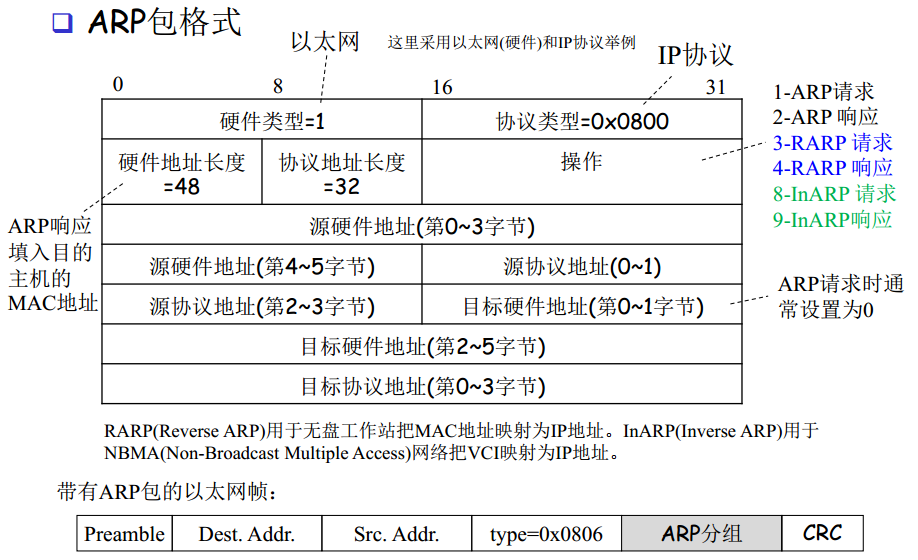
\includegraphics[width=0.7\linewidth]{fig/ARP.PNG}
\end{figure}

DHCP协议(Dynamic Host Configuration Protocol)用于主机在加入网络时\textbf{动态租用}IP地址,用UDP,四个步骤如下
\begin{itemize}
	\item DHCP发现(discover)
	\item DHCP提供(offer)
	\item DHCP请求(request)
	\item DHCP确认(ACK)
\end{itemize}

因特网控制消息协议(Internet Control Message Protocol, ICMP)用于主机或路由器发布网络级别的控制消息,主要是出错/丢包后将信息发回给源主机(TTL减到0、不可达),如回响请求和答复消息(ping)、不可达消息、时间超时消息(原IP头部+原IP数据部份的头64B)、重定位消息

% Path MTU Discovery 用于寻找路径上最小MTU
% Traceroute 用于获得整条路径上的路由器IP地址
% 交换机端口镜像Port Mirroring, also known as SPAN (Switched Port Analyzer) 实现监听
% DHCP Relay(中继) 多个局域网共享一个DHCP服务器 https://www.netmanias.com/en/post/blog/6004/dhcp-network-protocol/what-is-a-dhcp-relay-agent

\subsection{路由协议}
有类网的路由选择算法:
利用数据包中的\textbf{目的地址}得到\textbf{目的网络号},然后查询\textbf{路由表}(routing table)/转发表(forwarding table)
\begin{itemize}
	\item 如果查询的结果为\textbf{直连网},则\textbf{下一跳(next hop)为空},直接把数据包从查出的接口转发到目的主机
	\item 否则,如果查询得到\textbf{下一跳}(路由器),则把数据包转发给下一跳
	\item 如果没有查到任何匹配项,则把数据包转发给\textbf{默认路由器}(也算查到)
	\item 如果没有设置默认路由,则\textbf{丢弃}该数据包
\end{itemize}

无类网的路由选择:
无类网的路由表里有子网掩码
\begin{itemize}
	\item 匹配方法: 目的IP地址 \& 子网掩码 $==$ 子网号
	\item 最长匹配原则(The longest match rule): 当有多条路由都匹配时选择子网掩码最长(1的长度)的路由,因为更详细
	\item 从IP数据报中获取目的地址,利用目的地址\textbf{查路由表}(同有类网)
	\item 直连网将数据报直接\textbf{封装成帧}发送,不需要目的地址(PPP)
	\item 以太网同样要封装成帧,从\textbf{路由表中查出下一跳}的IP地址,通过\textbf{ARP协议}获得\textbf{目的MAC地址},加入帧内
	\item 如没有下一跳,则直接取\textbf{IP数据报中的目的IP地址}(已经到达了)
	\item 发送时要遵守以太网协议(CSMA/CD)
	\item 每到一个路由器都将帧拆出来,再重新封装,目的和源MAC地址(上一跳路由器MAC地址)全要发生变化
\end{itemize}

路由表
\begin{itemize}
	\item 127.0.0.1是内部的,其他是外部的需要经过防火墙
	\item 接口不一样,因此要在路由器里写两项,一项内部一项外部
	\item 往外发,默认路由会匹配
	\item 选择跃点数(metric)小的一项,如果跃点数也相同,则两个接口都会发送
\end{itemize}
% 点到点可以路由器端口不用配IP地址,但以太网一定要配,因为可能有交换机

路由表可以由管理员手工建立,也可以由路由/路由选择协议(routing protocols)自动建立。
路由协议即自动建立路由表,包括网络号、子网号、下一跳、接口、开销等。
所建立的路由分别称为\textbf{静态路由}和\textbf{动态路由}。
默认路由和直连路由都是静态路由。

建路由表是记\textbf{最短路径}的下一跳。

整个因特网实际上由很多机构进行管理。每个机构管理自己的网络,它们有权决定采用什么协议和网络控制策略。这样在\textbf{同一个机构}管理下的网络称为一个\textbf{自治系统}(autonomous systems, AS)。因特网实际上是由很多自治系统构成的。
\begin{itemize}
	\item 用于在AS\textbf{内部}(Intra-AS)建立动态路由的路由协议称为\textbf{内部网关协议}(Interior Gateway Protocols, IGP)。例如,\underline{RIP协议}和\underline{OSPF协议}。一个AS通常运行单一IGP。
	\item 用于在AS\textbf{之间}(Inter-AS)建立动态路由的路由协议称为\textbf{外部网关协议}(Exterior Gateway Protocol, EGP)。例如,\underline{BGP协议}。
	\item 运行同一个IGP协议的连通区域也称为路由选择域(routing domain)。一个AS可以运行多个IGP协议,形成多个路由选择域。
\end{itemize}

加了网关相当于加了默认路由。

网络层在入口位置有防火墙,未查路由表就丢弃了。

路由算法(Routing algorithm):路由协议里用的算法, 由于两个路由器之间都有开销,可以建立一个图,找最短路径
\begin{itemize}
	\item 链接状态(link state, LS):Dijstra
	\item 距离向量(distance vector, DV):BellmanFord
\end{itemize}

\subsubsection{RIP协议}
路由信息协议(Route Information Protocol, RIP):\textbf{距离向量}算法的路由协议(问路),工作原理是\underline{采用邻居的路由表构造自己的路由表}。
\begin{itemize}
	\item 每\textbf{30秒}\footnote{太频繁会占用带宽}RIP路由器把它的整个路由表发送给邻居。具体实现时每个邻居会错开发送,30秒的时间也会随机变化一点。
	\item 初始时每个RIP路由器只有到直连网的路由,它们的距离为1。
	\item 到目的网络的距离以跳为单位。最大距离为15。距离16表示无穷大,即目的网络不可达。
\end{itemize}

具体算法:
当收到邻居发来的路由表(update packet),路由器将更新它的路由表$\lrang{\text{目的网络},\text{开销},\text{下一跳}}$:
\begin{enumerate}
	\item 收到路由的距离全部加1(即一跳的距离)
	\item 利用上述路由修改路由表:
	\begin{itemize}
		\item 把路由表中不存在的路由加入路由表
		\item 如果比路由表中的路由的距离更小,则更新该路由的距离为新距离,把下一跳改为邻居。如果原来的更大,则\textbf{也要进行改动},因为原来的路可能断了。即路由的下一跳送来的新路由,则必须修改距离。
	\end{itemize}
	\item 如果路由存在,就要重置失效定时器
\end{enumerate}
RIP路由表的每一项都有TTL(Time-To-Live),用失效定时器(invalid timer)计时,超时则让该路由失效

RIP协议存在的问题
\begin{itemize}
	\item 慢收敛:最短时间接近$0$(这样看更新时刻),最长时间$30(m-1)$,平均时间$15(m-1)$
	\item 计数到无穷:N1-R1通路断了,R1收到R2的路由表,更改自己的
\end{itemize}

RIP协议的技术
\begin{itemize}
	\item 水平分割(split horizon)技术:从一个接口学来的路由不会从该接口发回去;依然会计数到无穷,三角形R1断了,R1先发,R2后发
	\item 毒性反转(poison reverse)技术:当一条路由变为无效之后,路由器并不立即将它从路由表中删除,而是将其距离改为用16后广播给邻居,使邻居所拥有的该路由立即失效,而不是等待TTL到期后删除,以迅速消除路由环路,这种方法称为毒性反转,距离为16的路由称为毒化路由(poisoned route)
	\item 抑制技术(hold down):距离被改为无穷大的路由在一段短时间(180秒)内其距离不允许被修改
	\item 触发更新(triggered update):一旦出现路由变化将立即把变化的路由发送给邻居。原有的30秒发一次完整的路由表依然不变
\end{itemize}

RIP协议简单、容易实现。特点如下
\begin{itemize}
\item 网络的直径不能超过16跳
\item 不允许把一个大网络分成多个区
\item 开销缺乏灵活性
\item 存在慢收敛问题和计数到无穷问题
\item 每30秒发送完整路由表会消耗大量的带宽
\item 实际运行的RIP协议具有如下特性:
\begin{itemize}
\item 可以保存多达6个等距离的路由在路由表中,默认为4个
\item 直连网的管理距离为0,RIP协议的距离为1
\end{itemize}
\end{itemize}

\subsubsection{OSPF协议}
开放最短路径优先协议(Open Shortest Path First, OSPF)采用\textbf{链路状态}路由算法,可能是在大型企业中使用最广泛的内部网关协议:
\begin{itemize}
	\item 利用最短路径算法,如Dijkstra,求出一个节点(源节点)到所有其它节点的最短路径
	\item 利用这些最短路经上的下一个节点作为下一跳得到源节点的转发表(路由表)
\end{itemize}

OSPF协议的简单描述:
\begin{itemize}
\item 周期性地收集链路状态,并扩散给AS中的所有路由器
\item 用收到的链路状态建立整个AS的拓扑结构图
\item 利用Dijkstra算法计算到AS中所有网络的最短路径
\item 利用这些路径上的下一跳建立路由表
\end{itemize}

OSPF第一步需要将整个网络(AS)转化为AS的拓扑结构图。
\begin{itemize}
	\item 每一个路由器和每一个网段(多路访问网络/\textbf{点到点网络})都作为一个结点
	\item 每个中转网(transit network),要选举一个直连路由器作为其指定路由器(designated router, DR)
	\item 中转网只有入边有权,出边都没有
	\item 如果点到点网络没有配置IP地址,则该结点可去除
	\item 末端网(stub network)即不再连其他路由器的网络
	\item 每一个路由/网段都有自己的链路状态通告(Link State Advertisement, LSA)
\end{itemize}

详细过程如下
\begin{itemize}
	\item 发现邻居:每10秒向邻居发送Hello分组,如果40s(dead interval)都收不到邻居发来的Hello分组,则把到邻居的链路标记为失效。多路访问网络采用多播(224.0.0.5, all OSPF routers)发送Hello分组。一个Hello分组包含优先权、已知的邻居(收到过Hello)、DR和BDR
	\item 完全相邻:在发现邻居之后, OSPF路由器将与邻居交换链路状态数据库中的LSA,请求得到更新的或者没有的LSA。在与邻居的链路状态数据库变得完全一样时,它们就处于完全相邻状态(fully adjacency)
	\item 生成LSA:每30分钟或链路变化时,每个OSPF路由器会生成router LSA,中转网的DR会生成	network LSA
	\item 扩散LSA:产生的 LSA立即封装为Update分组,被可靠地扩散出去 (需要确认)。每次产生的LSA的序号会加1。序列号越大表示越新。若通过收到多个LSA,由发出此LSA的路由器ID(发通告路由器),链路状态和序列号唯一确定。通过序号,也可以防止扩散形成回路,第二次收到来自相同的发通告路由器、相同LSA类型和相同序号的LSA将丢弃它
	\item 收集LSA:路由器收集到LSA之后,用新LSA替换链路状态数据库中旧LSA。如果一个LSA在60分钟(max age)没有被更新,它将从链路状态数据库移除
	\item 计算最短路径:当链路状态数据库被改变时, OSPF路由器将利用Dijkstra算法计算到所有网络的最短路径。
	\item 建立路由表:利用得到的最短路径产生路由表
\end{itemize}

OSPF协议采用路由器ID(RID)标识每一个路由器。
路由器ID由以下方法得到:
\begin{itemize}
	\item 使用直接配置的RID
	\item 所有活动环回接口中最大的IP地址
	\item 所有活动物理接口中最大的IP地址
\end{itemize}
除非路由器重启、所选接口故障或关闭或IP地址改变、重新执行了router-id命令,RID都将保持不变。

% 透明网桥来了就转,数据报中没有标识
% 但对于OSPF来说,有序号,知道收到过一次,就把它丢了,管理数据所以可以这样弄

指定路由器
\begin{itemize}
	\item 当多路访问网络重启时,选择DR的过程就开始了。在等待时间结束(Wait Time/Dead Interval, 40s)时,带有最高和次高优先权的路由器分别成为DR和BDR(Backup DR)。如果优先权相同,RID更大的成为DR,次大的成为BDR。
	\item 如果路由器不希望参与选举,则应该把优先权设置为0。如果优先权相同,具有更高RID的路由器成为DR。如果收到的Hello列出了DR(RID不是0.0.0.0),路由器成为DR。
	\item 如果一个新的路由器在选举之后到达或者有路由器修改为更高的优先权,它也不可能抢占现存的DR/BDR和变为DR/BDR。
	\item 当DR失效时, BDR成为DR,将开始一个新的选举过程来选出BDR。
	\item 一个多路访问网络中的OSPF路由器只与DR和BDR建立相邻关系。
	\item 收到一个LSA后,一个多路访问网络中的OSPF路由器将把它首先多播(224.0.0.6)给DR和BDR,然后 DR再把它多播(224.0.0.5)给所有OSPF路由器
\end{itemize}

LSA具有多个定时器
\begin{itemize}
	\item 每10秒(Hello Interval)向邻居发送一次Hello,4倍的hello interval(Dead Interval,40s)没有收到邻居的Hello就认为邻居失效。
	\item 每30分钟会产生新的LSA,最小间隔时间为5s。
	\item 每个LSA都有年龄字段(age),发给邻居时被设置为0,在链路状态数据库中age会不断增长,增长到Max Age(默认为60分钟)时LSA被标记为失效。失效的LSA会被扩散到整个AS,令AS的所有路由器把该LSA从链路状态数据库中移除。
	\item 存储在链路状态数据库中的LSA每10分钟会被计算校验和,如果有错将被删除。
	\item 接收来自邻居的LSA的最小间隔时间为1s。
	\item 计算最短路径的最小间隔时间为10s。
\end{itemize}

OSPF特点
\begin{itemize}
	\item 所有的OSPF消息都要认证 (防止恶意入侵)。
	\item 路由表中允许多个\textbf{相同开销}的路经存在(RIP只允许一条路径),可以实现负载均衡。
	\item 对于每条链路,允许同时有多个(TOS)开销。
	\item 多播OSPF(MOSPF)使用与OSPF相同的链路状态数据库(思科路由器不支持)
	\item 在大型路由选择域中OSPF可以\textbf{分区}。
	\item 比RIP\textbf{收敛快而且更安静}。
	\item 实现起来更复杂,需要更多的\textbf{计算开销}。
\end{itemize}

LS算法和DV算法比较
\begin{center}
\begin{tabular}{|c|c|c|}\hline
	& LS & DV\\\hline
消息复杂性 & n个节点, E条链路, 要发送$O(nE)$条消息 & 只在邻居之间交换消息\\\hline
收敛速度 &
\begin{tabular}{l}
$O(n^2)$算法需要$O(nE)$条消息\\
可能会震荡
\end{tabular} &
\begin{tabular}{l}
收敛时间变化\\
可能出现路由循环\\
计数到无穷问题
\end{tabular}\\\hline
健壮性\footnote{路由器失效时会出现什么情况?} &
\begin{tabular}{l}
可能通告不正确的链路开销\\
每个节点只计算自己的路由表
\end{tabular} &
\begin{tabular}{l}
DV节点可能通告不正确的路径开销\\
每个节点的路由表被其它节点所用\\
错误会通过网络传播开
\end{tabular}\\\hline
\end{tabular}
\end{center}